\documentclass[a4paper,11pt]{article}
\usepackage[utf8]{inputenc}
\usepackage{lastpage}
\usepackage{fancyhdr}
\usepackage[english]{babel}
\usepackage[a4paper,margin=1in]{geometry}
\usepackage{multirow}
\usepackage[table,xcdraw]{xcolor}
\usepackage{array}
\usepackage{graphicx}
\usepackage{caption}
\usepackage{ctable}
\usepackage{listings}
\usepackage[T1]{fontenc}
\usepackage{bigfoot} % to allow verbatim in footnote
\usepackage[numbered,framed]{matlab-prettifier}
\usepackage{amsmath}


\newcolumntype{L}[1]{>{\raggedright\let\newline\\\arraybackslash\hspace{0pt}}m{#1}}
\newcolumntype{C}[1]{>{\centering\let\newline\\\arraybackslash\hspace{0pt}}m{#1}}
\newcolumntype{R}[1]{>{\raggedleft\let\newline\\\arraybackslash\hspace{0pt}}m{#1}}

\newcommand\tab[1][4mm]{\hspace*{#1}}


%-------------------------------------------------------------------------------
% HEADER & FOOTER
%-------------------------------------------------------------------------------

\pagestyle{fancy}
\fancyhf{}
\setlength\headheight{15pt}
\fancyhead[L]{ Imaging Lab 5 }
\fancyhead[R]{Student ID: 100633486}
\fancyfoot[R]{Page \thepage\ of \pageref{LastPage}}


%-------------------------------------------------------------------------------
% TITLE PAGE
%-------------------------------------------------------------------------------

\begin{document}

\title{
	\Huge \textbf {The Calculus of Images}
    \\ [0.2cm]
	\LARGE Imaging Lab 5 - May, 2017
    \\ [0.5cm]
    \hrule
}

\date{}

\author{
		\Large Kamyar Nazeri \\
		\large Student ID: 100633486 }

\maketitle
\newpage

\section*{Curvature Matrix of an Image}
In this assignment, we are writing a Matlab function to compute the curvature matrix of an input grayscale image. The function takes a grayscale image as an input argument, computes first and second derivative of image and returns a the curvature matrix. \\
The curvature \emph{k} (and the discredited approximation) shown below measures the rate at which the unit gradient vector is changing:
\begin{align*}
  k = \nabla \cdot \bigg(\frac{\nabla u}{\Vert\nabla u\Vert}\bigg) \approx \frac{u_{xx}u_y^{2} - 2u_xu_yu_{xy} + u_{yy}u_x^{2}}{(u_x^{2} + u_y^{2})^{3/2}}
\end{align*}
\\
\emph{Listing 1} shows the Curvature function's implementation in Matlab:

\begin{lstlisting}[caption={Matlab Curvature Function},captionpos=b,style=Matlab-editor]
function k = Curvature(img)
    % Computes the curvature matrix of an input grayscale image

    a = 0.01;               % fudge factor
    [m,n] = size(img);      % image size
    img = double(img);      % convert input image to double

    % u_x = (u(x+1,y) - u(x-1,y)) / 2
    u_x = (img(:,[2:n,n]) - img(:,[1,1:n-1])) / 2;

    % u_y = (u(x,y+1) - u(x,y+1)) / 2
    u_y = (img([2:m,m],:) - img([1,1:m-1],:)) / 2;

    % u_xx = u(x+1,y) - 2u(x,y) + u(x-1,y)
    u_xx = img(:,[2:n,n]) - 2 * img + img(:,[1,1:n-1]);

    % u_yy = u(x,y+1) - 2u(x,y) + u(x,y-1)
    u_yy = img([2:m,m],:) - 2 * img + img([1,1:m-1],:);

    % u_xy = (u(x+1,y+1) + u(x-1,y-1) - u(x-1,y+1) - u(x+1,y-1))/4
    u_xy = (img([2:m,m],[2:n,n]) + img([1,1:m-1],[1,1:n-1]) -   img([2:m,m],[1,1:n-1]) - img([1,1:m-1],[2:n,n])) / 4;

    % multiplications and powers are all componentwised
    k_num = (u_xx.*u_y.^2) - 2*(u_x.*u_y.*u_xy) + (u_yy.*u_x.^2);
    k_denom = (u_x.^2 + u_y.^2).^(3/2) + a;

    % componentwise division
    k = k_num ./ k_denom;
end
\end{lstlisting}

\newpage

\emph{Figure 1} shows a test image and its curvature matrix side-by-side. The curvature is zero in flat regions and along straight edges; however it is visible along the perimeter of the circles and the edges of the square: 

\begin{figure}[!htb]
  \centering
  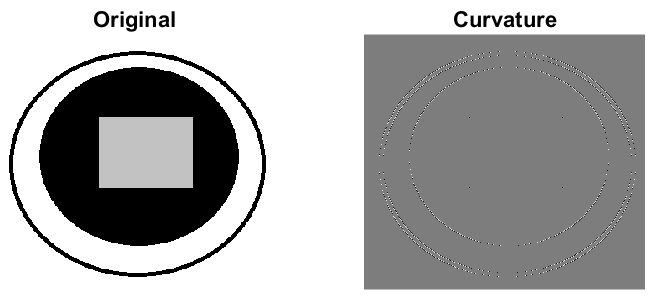
\includegraphics[width=14cm, height=6.5cm]{1.png}
  \caption{\small Curvature image of a grayscale test image}
\end{figure}

\end{document}
